\chapter{Contribution Quality}
\label{ch:editquality}

\begin{quote}
\textit{
This chapter expands on ideas originally
described in~\cite{Adler2007}.}
\end{quote}

%\mynote{Make sure to not use term \textit{metric}!  It
%has a specific definition that our edit distance does not
%meet.  Correct phrase seems to be \textit{similarity measure}.}

\section{Introduction}

The problem with modern research trends (Google Pagerank, Netflix
prize, etc) is that we're pursuing human ideas of ``good''.
There is no gold standard, no way to prove correctness except
by example and rhetoric.
This research has the same problem, though we've tried to address
that by having human evaluations and other measures.

The problem of evaluation is also a matter of quality, or at least
putting a quantity on the quality.
In our original work, we propose several ways to do evaluation.
Vandalism includes several different kinds of evaluation.
Problem in our field is that nearly no one does head-to-head
comparisons, so it's legitimate to post some precision/recall
numbers that ``look good'' and then be done with it.

Working in industry, evaluation is also the first thing tossed
out the window in the rush to file patents or create demos.


\section{Related Work}
\label{sec:vandalism-related}

Wikipedia's official statement of vandalism defines it as
``a \textit{deliberate} attempt to compromise the integrity
of Wikipedia.''\footnote{
\url{http://en.wikipedia.org/wiki/Wikipedia:Vandalism}}
It is, of course, impossible to know the motivations of individuals,
so this definition relies on human intelligence to determine
vandalism on a case-by-case basis --- that is, ``I know it
when I see it,''\footnote{Justice Potter Stewart in
\underline{Jacobellis v. Ohio}, 378 U.S. 184 (1964)}
but there is no precise definition.
Some researchers have undertaken the task of more formally defining a
taxonomy of vandalism~\cite{Viegas2004,Priedhorsky2007,Chin2010},
but nearly all research on vandalism detection uses one of a small
number of (convenient) definitions for purposes of obtaining an
annotated corpus: \textbf{manual annotation} uses human intelligence
to infer the intentions of the
editor~\cite{Potthast2008,Chin2010,West2010,Potthast2010a},
\textbf{reverts} are notations by the community when it feels that
vandalism has taken place~\cite{Smets2008,Itakura2009,Belani2010},
\textbf{rollbacks} are disapprovals by Wikipedia
Administrators~\cite{West2010},
and \textbf{edit quality} generalizes the idea of measuring the
sentiment of the community~\cite{Adler2007,Druck2008}.
There is an obvious trend going from \textit{manual} to
\textit{automatic} annotation, but equally important is to observe
that there is a trend from external judgement, to internal explicit
judgement, to internal implicit judgement.
Ultimately, it is the community itself which decides what is
vandalism (\eg the stark contrast between the communities of
Slashdot\footnote{\url{http://slashdot.org}} and
Hacker News\footnote{\url{http://news.ycombinator.com}}),
and this community standard is likely to change over time
(often described as the ``signal-to-noise'' ratio of the community;
examples of changing communities include USENET and Slashdot).
This argues strongly in favor of automated methods for measuring
the reaction of the community, and highlights the idea that vandalism
detection is a specialized form of trying to measure the ``noise'' in
a community.

The earliest attempts at vandalism detection within the Wikipedia come
directly from the user community and try to encode a human intuition
of vandalism detection into an expert system (some examples
include~\cite{wiki:AntiVandalBot,wiki:MartinBot,wiki:ClueBot,Carter2007}).
The largest disadvantage to this class of solution is that building
an expert system requires extensive human labor to produce the manual
annotation and analysis required to derive custom rules from the
annotation.
Primarily, the rules developed are based on features of the actual
content of the edit rather than on metadata (\eg an edit containing
only capital letters is indicative of vandalism).

The idea that the content is the primary source of features that
reveal the intent of the author is a natural one, and is investigated
by several different research groups
(\eg~\cite{Potthast2008,Smets2008,Druck2008,Itakura2009,Chin2010}).
Casting the problem as a machine learning binary classification
problem, Potthast~\etal~\cite{Potthast2008} manually identify and
inspect 301~incidents of vandalism to generate a feature set based on
metadata and content-level features and build a classifier using
logistic regression.
Smets~\etal~\cite{Smets2008} applies the ``naive bayes'' machine
learning technique to a bag-of-words model of the edit text.
Chin~\etal~\cite{Chin2010} delve deeper into the field of
natural language processing by constructing statistical language
models of an article from its revision history.
(On the topic of manual annotation, they also describe how supervised
active learning can help the training process by requesting
annotations for examples which will make a significant difference to
the algorithm.)

A different way of looking at the content approach is the
realization that appropriate content somehow ``belongs together,'' and
one way to measure that is through compression of the successive
revisions of an article~\cite{Smets2008,Itakura2009}.
If inappropriate content is added to the article, then the compression
level is lower than it would be for text which is similar to text
already in the article.
This is much more powerful than the bag-of-words model, because
phrases are significant and lead to better compression; nonsensical
sentences that include some key words will not compress as well.
A significant drawback of these compression techniques is that they
require manipulation of the content of a large number of revisions
from the article being edited.

Content-based analysis has the burden of having to
inspect potentially large edits, but the alternative is to depend
on the paucity of information available in the metadata ---
many previous works have some small dependence on metadata
features~\cite{Potthast2008,Druck2008,Belani2010}, but only
as far as it encoded some aspect of human intuition about vandalism.
Drawing inspiration from other areas of research,
West~\etal~\cite{West2010} demonstrate astonishing results because
they are based entirely on metadata (some of which is processed into
\textit{reputations}) that indicate there is more relatedness between
vandals than is readily apparent to the human eye.
One particularly interesting result was that using IP geolocation
to cluster users leads to better predictions, presumably because
anti-US sentiment also tends to cluster by geographic region.

The first systematic review and organization of features appears
by Potthast~\etal~\cite{Potthast2010b} as part of the competition
associated with the PAN~2010 Workshop on vandalism
detection.
Belani~\cite{Belani2010} includes several metrics for evaluating
predictors, and Potthast~\etal take up the discussion with a thorough
comparison of nine competitors using both the area under the
precision-recall curve and the area under the receiver operating
characteristic curve.
Potthast~\etal conclude their analysis by building a meta-classifier
based on the nine entries and discover that the result performs
significantly better than any single entry.

User reputation systems~\cite{Zeng2006,WikiMTWtrust06,Adler2007}
have been previously proposed as an underlying technology for
vandalism prevention or detection, and the second place entry in
the PAN~2010 competition was a system based on the
WikiTrust project~\cite{Adler2010b}.
In that entry, the WikiTrust user reputation system was not
directly used as a feature due to not having a historical record
of the reputation values.
The work presented in this chapter extends~\cite{Adler2010b} by
tracking the historical user reputation values and using that
as an additional feature to the machine learning algorithms.

The winner of the PAN~2010 competition, by a notable margin, was
an entry by Mola-Velasco~\cite{Mola2010} that extended the features
originally proposed by Potthast~\etal~\cite{Potthast2008}.
This entry was composed of 21~features (the largest in the
competition) that comprehensively model the content of the edit,
including features that rated use of language, formatting of text,
compressibility with earlier text, spelling,
and the size of the edit.

The combining of features used by Mola-Velasco~\cite{Mola2010},
WikiTrust~\cite{Adler2010b} and West~\cite{West2010}
is explored in~\cite{Adler2011a}.
That work improves on earlier results, and categorizes features
according to the difficulty of analysis.



\section{Text Quality}
\label{sec:textquality}

When first approaching the topic of measuring the quality
of contributions made by users, our thinking (perhaps shaped
by some of the public discussion surrounding
contributions~\cite{Swartz2006} \mynote{Other references?})
focused on the text being added by users.
The basic assumption of a reputation system is that past performance
is a reliable indicator of future performance, so we were
asking the question ``does text added by some users \intro{survive}
longer than text by other users?''
Note that there are other possible measures of quality, for example:
what size is the contribution, what is the reading level of the text,
how good is the grammar, and does the text seem to be related to
the topic of the article.
We decided not to tackle these kinds of quality measures, both for
the difficulty of natural language processing, and because such
methods would require significant work for each language we wanted
to support.
Measuring survival has the advantage that it's relatively cheap to
compute, and works the same way across most languages.

To calculate how long a piece of text survives,
we need to track the authorship of
units of text\footnote{For the WikiTrust project, we opted to
use a granularity of words to reduce the computational requirements.},
and then compute authorship again in later
versions of the article to find those words with an
authorship dating back to the revision we are trying
to determine the quality of.

In Chapter~\ref{ch:diff}, we describe how to track text authorship
for the text in an article $\article{} \in \articles$.
Just tracking authorship isn't enough for tracking survival, since
we need to know what specific revision a word came from.
Let us define another recursive relation, like the definition
for $\txtauthor{}$ in Equation~\ref{eq:txtauthor},
which defines the revision that a word was first introduced.
As before, we recall
$\words{\version{n}} = \left[ w_1, w_2, \ldots, w_{l_n} \right]$, and let $0 < j \le l_n$ in the following:
\begin{equation*}
\txtsrcrev{\version{n}, j} =
    \begin{cases}
        \txtsrcrev{\version{k}, s}, & \text{ if }
        \match{\version{n}, j, \prevrevs{\version{n}}} = (\version{k}, s) \\
        n, & \text{ if there is no best match text. } \\
    \end{cases}
\end{equation*}
Now we can define the text survival of words to be the number of
words introduced in \version{m} that are still present in \version{n}:
\begin{equation}
\tsurv{\article{}}{m,n} = \left| \left\{ j \colon
    \exists j . \txtsrcrev{\version{n},j} = m \right\} \right| \\
\label{eq:tsurv}
\end{equation}

\subsection{Text Decay Quality}

Our goal, in the abstract, is to define some metric that we can compute for
revisions which quantifies some estimate of the \intro{quality} of the
revision.
There are many possible ways to define quality measures, which is the
subject of research on vandalism detection (see
Section~\ref{sec:vandalism-related} for background on that topic).
As an example, a simple quality measure would be the heuristic that
inappropriate words added as part of an edit would indicate that the revision
is of poor quality.

For the purposes of building a reputation system, we want a measure
which provides some insight into the community perception of the
quality of the edit.
Having defined the notion of text survival, a very simple quality measure
could be ``what fraction of the text added in a revision survives
ten revisions later?''
We discuss some variations of these quality measures in
Chapter~\ref{ch:contrib}, but present here one novel quality measure.

\begin{figure}[htbp]
\centering
\framebox{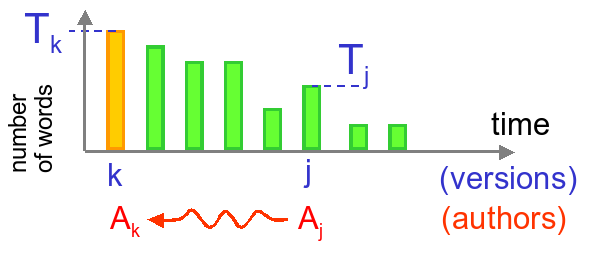
\includegraphics[width=0.9\textwidth]{part-F70-editquality/textcontr-2}}
\caption{A graphical depiction of how a text contribution survives
	through future revisions.
        An author, \editor{k}, adds
    $T_k = \tsurv{}{k,k}$ words in revision \version{k}.  In subsequent
    revisions, some of those words are deleted and partially restored.
    We say that a later author, \editor{j}, implicitly \intro{judges}
    author \editor{k} by choosing how many of \editor{k}'s words
    to keep or delete or restore; $T_j = \tsurv{}{k,j}$ is the number of words
    that were introduced in \version{k} that are still present, or
    \intro{live}, in \version{j}.
}
\label{fig:textsurvival} 
\end{figure}


In trying to understand how text contributions evolve, we decided
to limit our exploration to what happens to the text over the
following ten revisions.
Many contributions follow the simplest model: they are either
removed completely right away (a revert), or they are perfectly
preserved for the following ten revisions.
Some contributions, however, are only partially preserved, and
might even be partially restored as part of their evolution.
Figure~\ref{fig:textsurvival} gives a pictorial representation
of how some text introduced at revision \version{k} might
evolve over the next seven revisions; in this example, the
figure shows that some text was restored in revision \version{j}.
We say that author $A_j$ \intro{judges} the work of author
$A_k$ by deciding how much text to preserve, delete, and restore.
If author $A_j$ works on a different part of the article, she
is still implicitly deciding that the current revision of
$A_k$'s work is okay.\footnote{Some better model of
user attention would be useful for tempering the amount
of judgement we infer from
$A_k$ when they are focused elsewhere in the article.}

Measuring the fraction of text introduced in
revision \version{k} that survives to revision \version{j}
(\ie computing $\tsurv{}{k,j} / \tsurv{}{k,k}$)
gives useful information, but what if \version{j} happens to be
a vandal that blanks the page?
One idea would be to average the text survival over the next
several revisions (an idea explored in Chapter~\ref{ch:contrib}),
but we were struck by the observation that after some initial
churning, text seems to stabilize and then only slowly change
as time progresses.
We propose that a way to model this evolution of text over time
is as a geometric sequence with a common ratio between zero and one;
see Figure~\ref{fig:textlongevity} for how such a sequence could
approximate the text survival over several revisions.
The intuition behind a geometric model is that if an edit is
``bad,'' then most of the text will be removed right away.
As time passes, the size of the edits gets smaller and
the text tends to stabilize into a form
that people can agree on, until it eventually no longer changes.


\begin{figure}[tbph]
\centering
\framebox{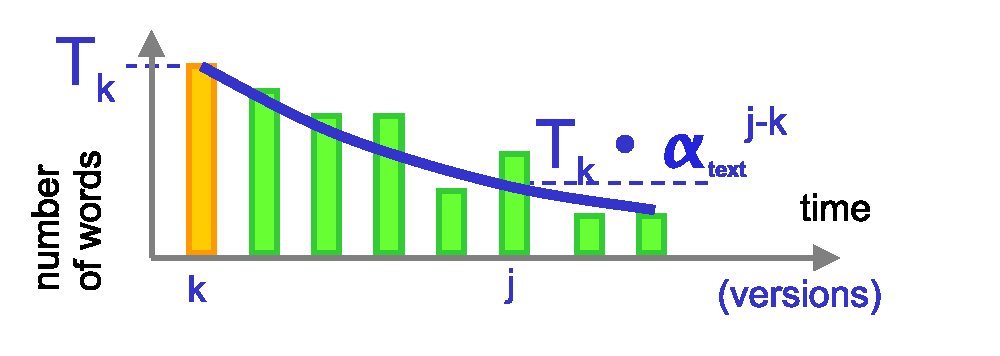
\includegraphics[width=0.9\textwidth]{part-F70-editquality/text-longevity}}
\caption{
    \mynote{Redo picture to change alpha to proper symbol.}
    To calculate the \intro{text longevity} of the contribution
    of $T_k$ words, we model the text survival as a geometric curve
    and compute a single number that describes how the text evolves
    over several revisions.}
\label{fig:textlongevity}
\end{figure}

\begin{figure}[tbph]
\centering
\framebox{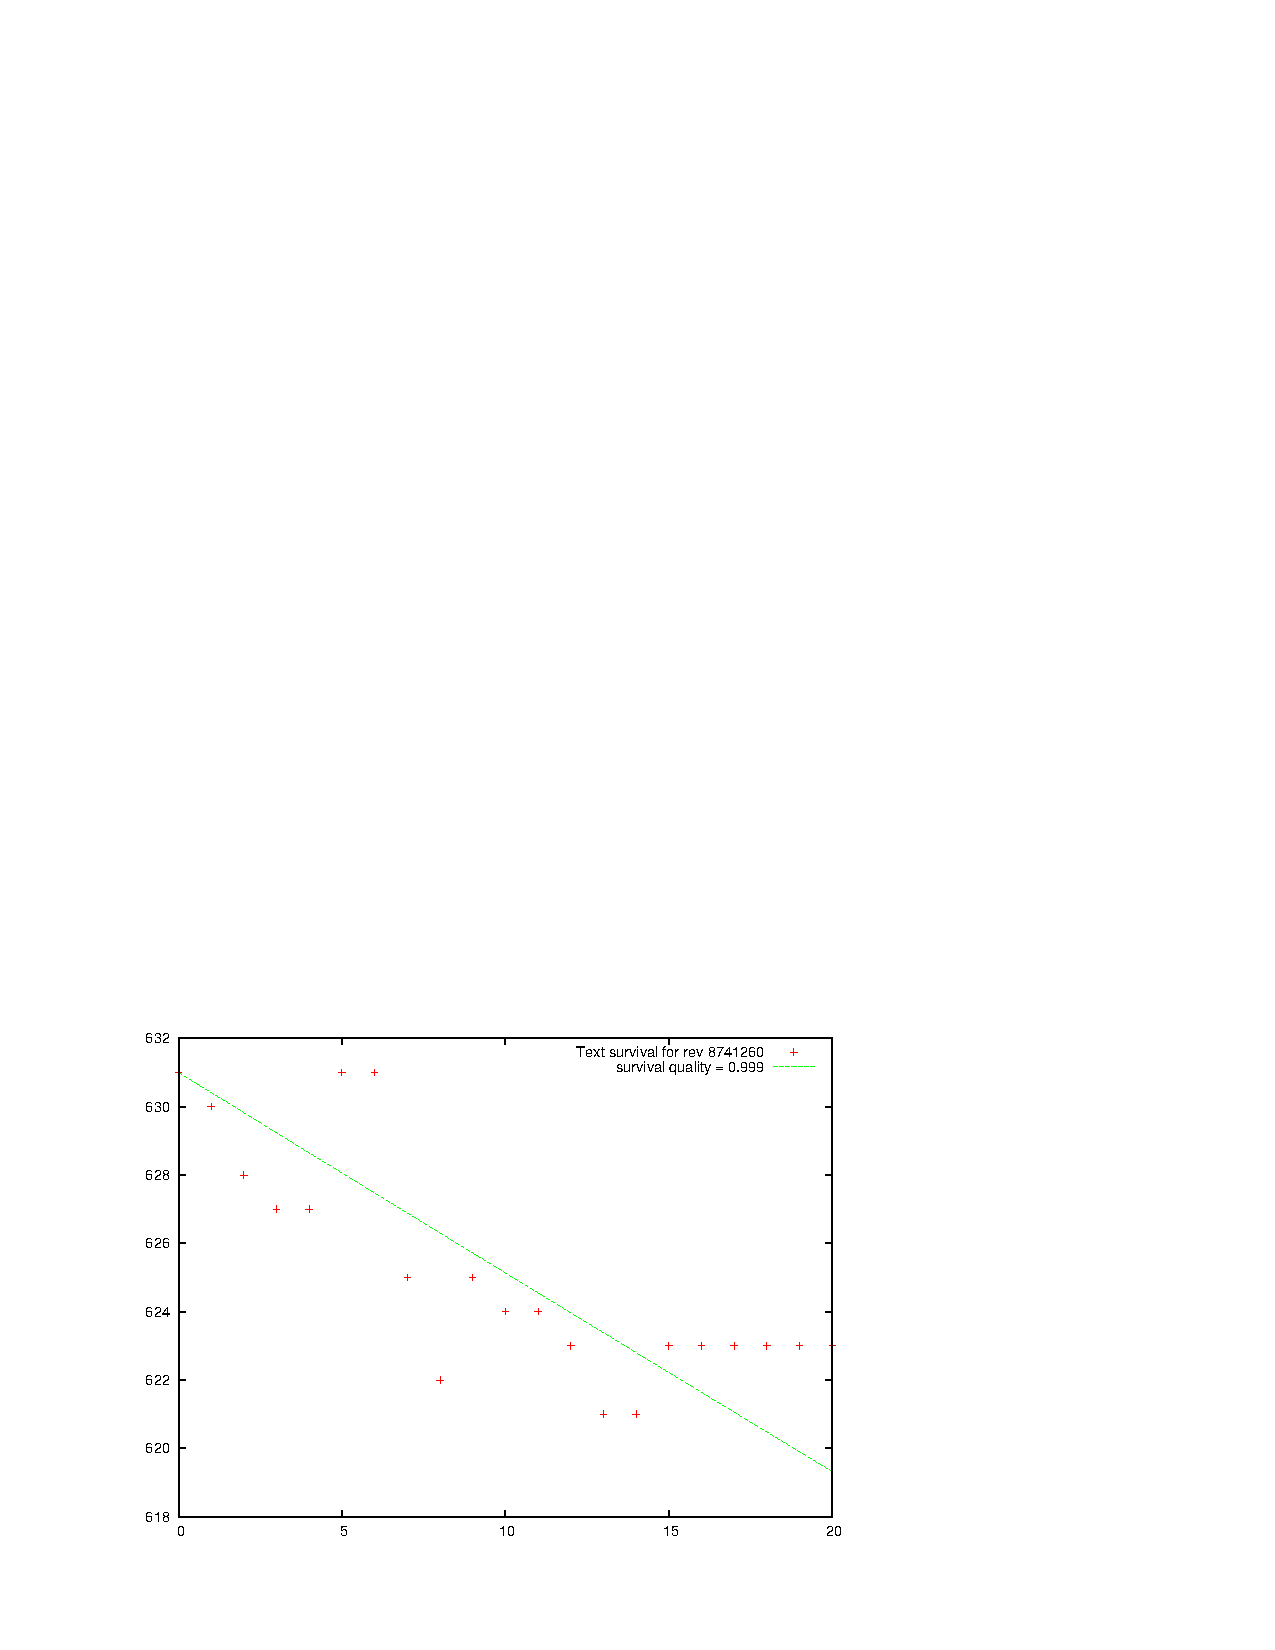
\includegraphics[width=0.95\textwidth]{part-F70-editquality/graph-TS-SantaCruzBeachBoardwalk}}
\caption{The text survival graph for the text initially contributed
	as part of the article \textit{Santa Cruz Beach Boardwalk}.
	The majority of the editing to the contributed text happens
	in the next few revisions, before the text stabilizes.
	Also shown in the graph is the text survival quality
	computed based on 20~revisions.
	}
\label{fig:ts-SantaCruzBeachBoardwalk}
\end{figure}

To measure the overall quality of a single text contribution
made in revision \version{k}, we need to compute the common ratio
that best describes the sequence of $n$ text survival values,
\tsurv{}{k,j}, after \version{k}, where $k < j \le k+n$.
Let us call this common ratio the \intro{text decay quality},
\quality{tdecay}{k}.
To compute \quality{tdecay}{k}, we want to solve the following equation:
\begin{align*}
    \sum_{i=0}^n \tsurv{}{k,k+i} = {} & \tsurv{}{k,k} + \quality{tdecay}{k} \cdot \tsurv{}{k,k+1} \\
    & + \quality{tdecay}{}{k}^2 \cdot \tsurv{}{k,k+2} + \ldots \\
    & + \quality{tdecay}{}{k}^n \cdot \tsurv{}{k,k+n} \\
    = {} & \tsurv{}{k,k} \cdot \sum_{i=0}^n \quality{tdecay}{}{k}^i \\
    = {} & \tsurv{}{k,k} \cdot \frac{1 - \quality{tdecay}{}{k}^{n+1}}{1 - \quality{tdecay}{}{k}} \\
\end{align*}

To solve this for \quality{tdecay}{}{k}, we can use Newton's method
to solve for the zero of the related function:
\begin{equation*}
  f(\alpha) = (1 - \alpha) \cdot \sum_{i=0}^n \tsurv{}{k,k+i}
        - (1 - \alpha^{n+1}) \cdot \tsurv{}{k,k}
\end{equation*}
where $\alpha = \quality{tdecay}{}{k}$.
Newton's method involves making repeated estimations of the form
\begin{equation*}
  \alpha_{j+1} = \alpha_j - \frac{f(\alpha_j)}{f'(\alpha_j)}
\end{equation*}
which we initiate with $\alpha_0 = 0$.
For efficiency reasons, we limit the number of iterations taken
to a small number (five in our live system)
since we are only estimating the quality and high precision
is not very useful.

The beauty of this quality measure is that it varies between
zero, for text which is immediately deleted, and one, for text
which is completely preserved.
Values in between the two extremes reflect the fact that there
was some debate among the community about what text to preserve
in the article.
Figure~\ref{fig:ts-SantaCruzBeachBoardwalk} shows the text survival
graph of the initial contribution to that article, and how it varies
over the next twenty filtered revisions.
The figure also shows the curve representing the decay quality,
calculated with a twenty-iteration Newton's method over the entire
twenty-one revision sequence.

\mynote{TODO: Still running author tracking on GWB page, redherring screen 2,
Sat, 5-Feb.}


\section{Edit Quality}
\label{sec:editquality}

The problem with measuring text contribution quality alone is that it
measures only one kind of user behavior: inserting and deleting of text.
Another important behavior of users is to rearrange text
(possibly with minor edits) so that it improves the flow or
readability of the text.
In traditional publishing, this is the role that the editor
serves, as opposed to the the author --- and both are valuable
to the quality of the final product.
Is there any notion equivalent to text survival for edits?
In struggling to answer this question, we first had to measure
the size of an ``edit contribution,'' which naturally led us to the
\intro{edit distance}~\cite{Levenshtein66,TichyEditDist,EditDistanceMoves,Adler2007}
metric.

Edit distance is typically used as a way to measure how many
insertions, deletions, and replacements are needed to transform
one string into another, and is thus defined as the sum of the
number of those operations.
Other formulations exist for edit distance, and within the
context of the WikiTrust project we were already computing
text differences as part of our author tracking algorithms,
so we chose to define the distance between two revisions
in terms of the edit script generated by our greedy text
matching algorithm.
The elements making up an edit script are:
\begin{itemize}
\item $\mathbf{Move}(i_1, i_2, k)$ -- a matching block of text of
    length $k$ words, starting at position $i_1$ in the source string,
    and position $i_2$ in the target string.
\item $\mathbf{Delete}(i, k)$ -- the text starting at position $i$
    and extending for length $k$ words was deleted from the source string.
\item $\mathbf{Insert}(i, k)$ -- the text starting at position $i$
    and extending for length $k$  wordswas inserted into the target string.
\end{itemize}
If we let $E(m,n)$ be the edit script set of elements describing the
transformation from the source string \version{m}
to the target string \version{n},
then we can define two terms for the total amount of insertions
and deletions by summing over all the matching elements:
\begin{align*}
  I_{tot}(m,n) =& \sum_{\exists i, k. \mathbf{Insert}(i, k) \in E(m,n)} k \\
  D_{tot}(m,n) =& \sum_{\exists i, k. \mathbf{Delete}(i, k) \in E(m,n)} k \\
\end{align*}
We then define the edit distance between revisions
\version{m} and \version{n} used within WikiTrust as
\begin{equation*}
    \dist{}{m,n} = I_{tot}(m,n) + D_{tot}(m,n)
        - \frac{1}{2}\min(I_{tot}(m,n), D_{tot}(m,n))
\end{equation*}
The motivation for this formulation of edit distance is
to try to account for replacements, which appear within
the edit script as insertion and deletions --- but the
position information required to match them is not preserved
by the difference algorithm.
By subtracting off a correction term, we make the assumption
that edits with both insertions and deletions make some
replacements which are being counted in both types of edit.

\subsection{Edit Longevity}

Given a method to measure the size of an edit contribution,
the problem still remains of how to compute whether that
contribution is preserved in future revisions.
An idea we considered is summing the edit distances of
sequential revisions, and comparing that against the edit
distance between the first and last revisions.
This has the problem that it roughly assumes that all
contributions are completely preserved or completely
reverted, but idea of mapping out the edit distances of
multiple revisions led to another idea that we favor.

Instead of trying to measure whether an edit is preserved,
let us ask the question, ``does this edit move us in the
direction of the future of the article, or does it move us away
from the future?''
This suggests consideration of three version: the one being
evaluated, one in the past, and one in the future.
Figure~\ref{fig-editcontr} visually represents the two possible
cases in evaluating revision \version{k}, using \version{k-1}
and \version{j} (where $j > k$) as guide posts for the general
path that the evolution of the article is taking.
If a contribution moves us in the general direction of
the future but has some extraneous text which is delete,
we get the case shown in Figure~\ref{fig-editcontr-a}:
the distance \dist{}{k,j} is smaller than the distance \dist{}{k-1,j}.
If the edit in \version{k} does not contribute at all to the
future of the article, then we have the case shown in
Figure~\ref{fig-editcontr-b}:
the distance \dist{}{k,j} is larger than the distance \dist{}{k-1,j}.

\begin{figure}[t]
\centering
\subfigure[Graphical representation of a good edit contribution.]{
\label{fig-editcontr-a} 
\framebox{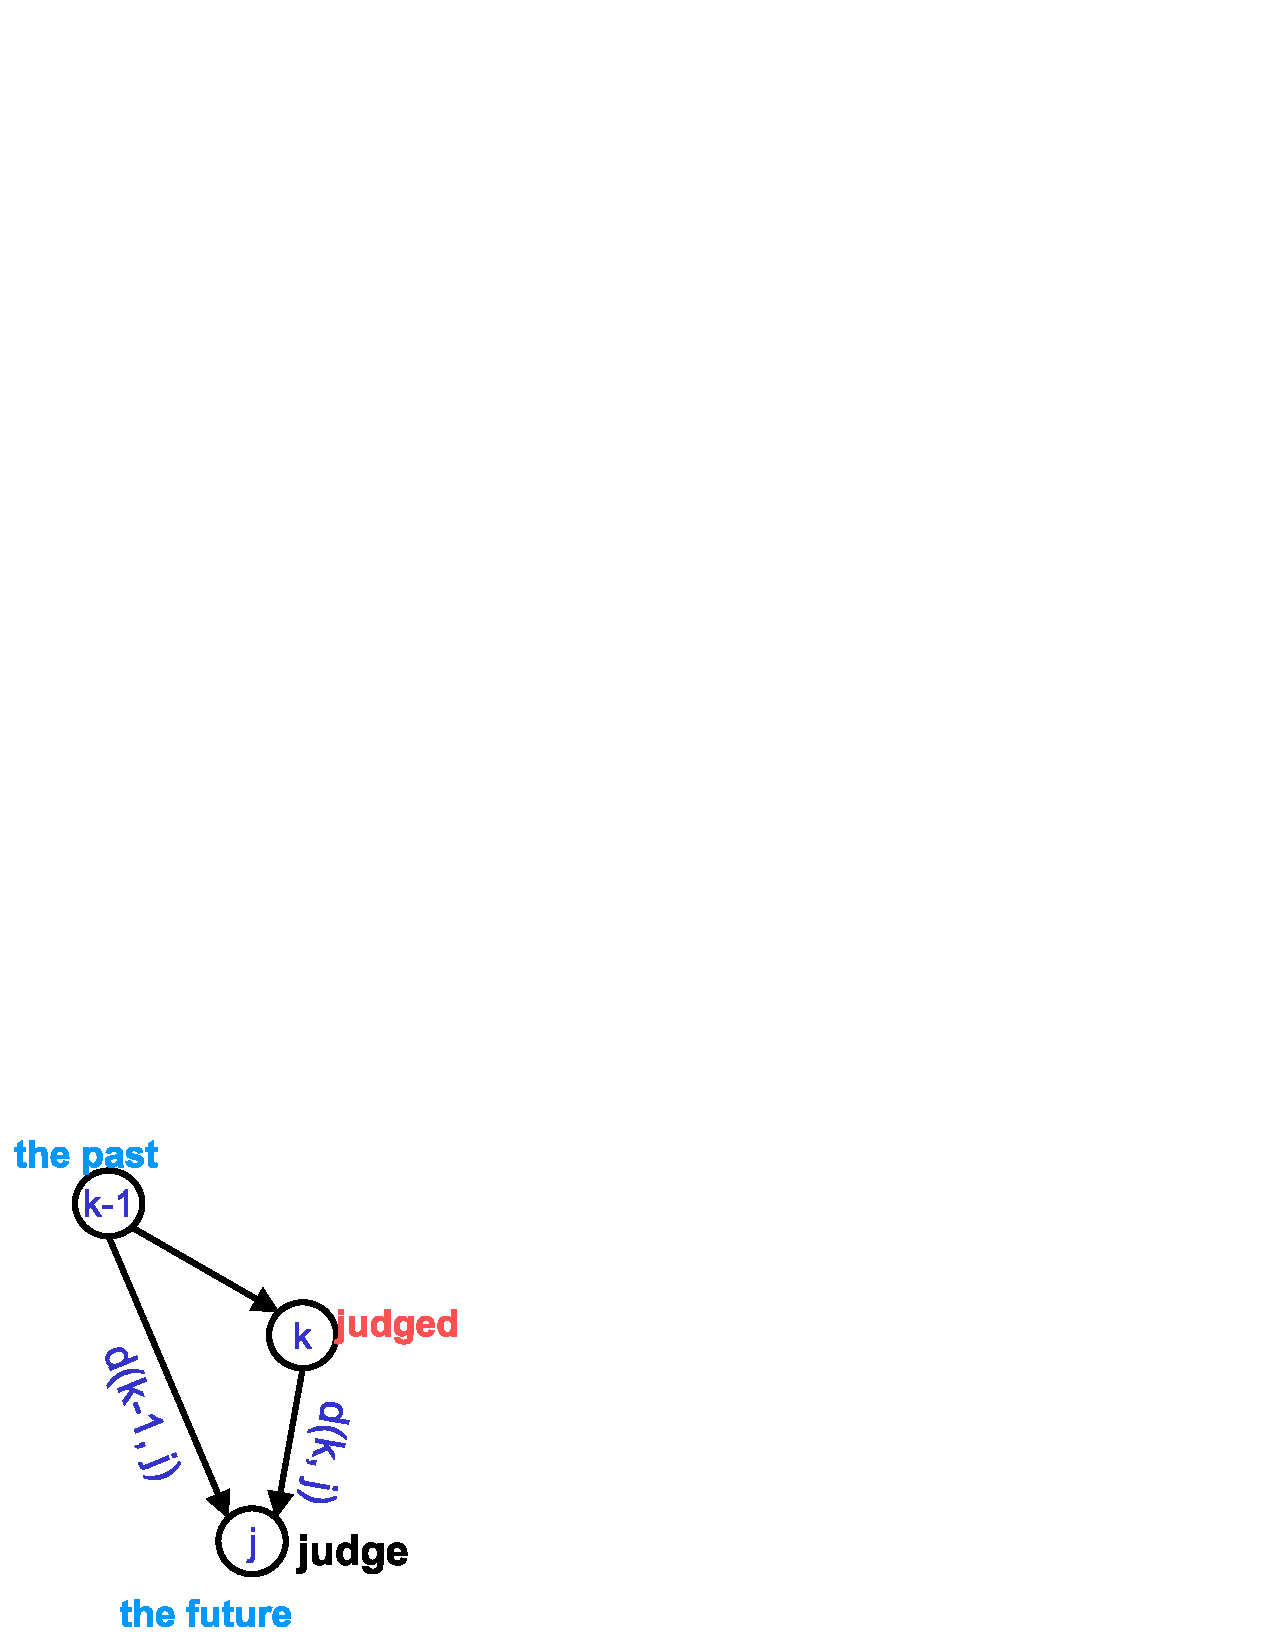
\includegraphics[width=0.35\textwidth]{part-F70-editquality/editcontr-good}}
}
\hspace{1ex}
\subfigure[Graphical representation of a bad edit contribution.]{
\label{fig-editcontr-b}
\framebox{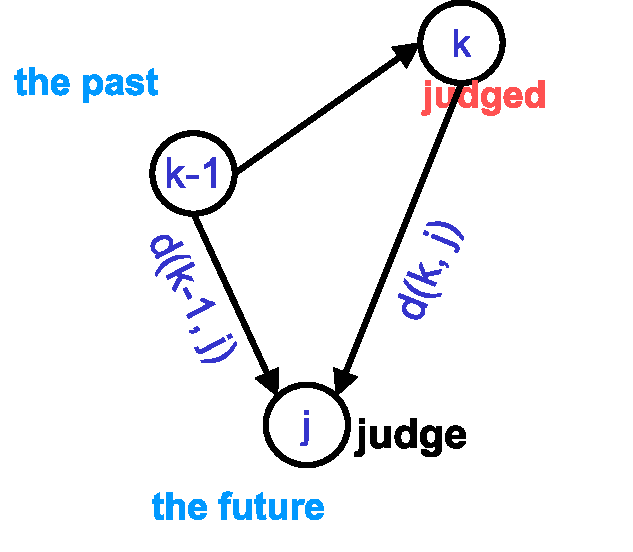
\includegraphics[width=0.40\textwidth]{part-F70-editquality/editcontr-bad}}
}
\caption{To measure the quality of version \version{k}, we also
	look at the previous version \version{k-1} and some future
	version \version{j}.
	The three versions form a triangle, using
	edit distance~\cite{Levenshtein66} to define the separation
	between each other.
	Intuitively, we know that when \version{k} is good,
	the distance to the future, $\dist{}{k, j}$,
	will be shorter than if \version{k} is bad.
	(When \version{k} is bad, more editing is required to
	bring it back to a better version, plus the editing
	to bring it to the future.)
}
\label{fig-editcontr}
\end{figure}

  To turn this into a quality metric for the
  version \version{k}, 
  we ask ``does the work done bring us closer to how the page
  will look in the future?''
  If future versions incorporate and build on the changes of edit \revision{k},
  then the edits are of good quality.
  When future versions mostly undo or discard the work of \revision{k},
  then the edits are of bad quality.

%\begin{wrapfigure}{r}{0.55\textwidth}
\begin{figure}
\centering
\framebox{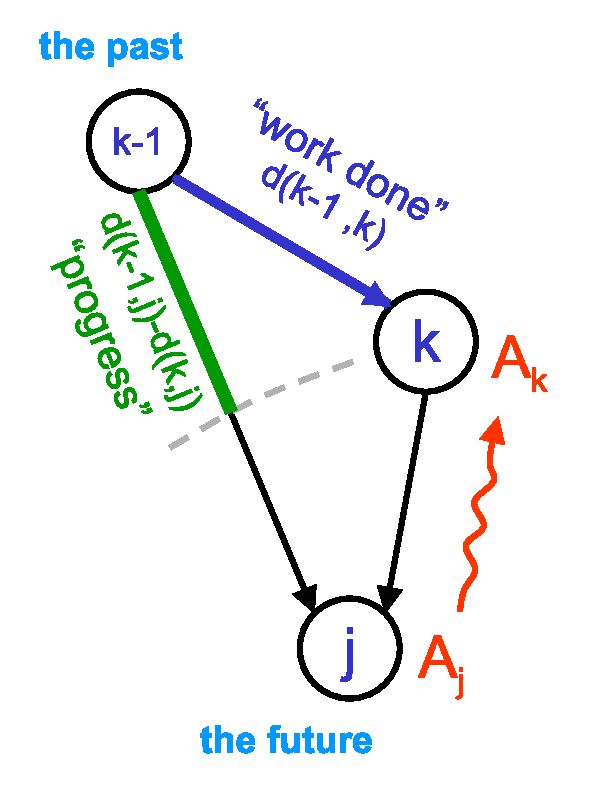
\includegraphics[width=0.35\textwidth]{part-F70-editquality/edit-longevity}}
\caption{Quality is measured by calculating how much \textit{progress}
	is made towards the future version of the article,
	and dividing that by the amount of \textit{work done}
	during the edit.}
\label{fig-editlong}
\end{figure}
%\end{wrapfigure}


  To calculate the quality of an edit \revision{k},
  we additionally consider two \intro{reference versions}:
  the immediate past \version{k-1} and some future version \version{j}.
  These three points allow us to define a triangle
  (see the two examples in Figure~\ref{fig-editcontr})
  using the edit distances $d(\version{k-1},\version{k})$,
  $d(\version{k-1},\version{j})$ and $d(\version{k},\version{j})$.
  We then computes the ratio
  \begin{equation*}
  \editq(\version{k},\version{j}) = \bigl[ \dist(\version{k-1},\version{j})
  		- \dist(\version{k},\version{j}) \bigr]
	/ \dist(\version{k-1},\version{k})
  \end{equation*}
  between the ``useful work''
  $\dist(\version{k-1},\version{j}) - \dist(\version{k},\version{j})$ and the
  ``total work'' $\dist(\version{k-1},\version{k})$
  (see Figure~\ref{fig-editlong} for a pictorial representation).
  The ``total work'' $\dist(\version{k-1},\version{k})$
  is a measure of how much change
  was performed during the
  edit $\revision{k}: \version{k-1} \goesto \version{k}$;
  the ``useful work''
  $\dist(\version{k-1},\version{j}) - \dist(\version{k},\version{j})$
  is a measure of
  how much closer the article becomes to the future version \version{j}.
  For reverted edits, the ratio $\editq(\version{k},\version{j})$
  is $-1$, since all of the work
  goes into \textit{increasing} the distance between \version{k} and \version{j}.
  For edits that are preserved, $\editq(\version{k},\version{j})$ is close to~1.
  The \intro{edit longevity}, \elong, of edit \revision{k} is then taken to
  be the average edit quality as judged by the next three revisions:
  \begin{equation*}
      \elong(\revision{k}) = \sum_{i=k+1}^{\min(k+3, n)}
      		\editq(\version{k},\version{i})
  \end{equation*}


\section{Evaluation Metrics}
\label{sec:rep-eval}

In developing a reputation system, one must ask
``what is it intended to signal?''
For WikiTrust, our hope was that a high reputation
would signal that edits made the author were likely
to be of good quality, while a low reputation would
signal that the edit was of unknown quality.
Evaluation of the system becomes the crucial
factor, so that users can compare one system to another.


At the time that this work was conducted, there was
no annotated corpus of edits available to compare against.
\mynote{Look up what McGuinness did for evaluation in her papers.}

We propose several different metrics for
evaluating our reputation systems, by casting the interpretation
into binary classification problems parameterized by a
quality metric.
We use the two quality metrics explored in Chapter~\ref{ch:editquality}
to define the following categories:
\begin{itemize} 
\item We say that the new text added in version \version{i}
  is \intro{short-lived} if $\quality{tdecay}{10}{i} \leq 0.2$.
  This indicates that at most 20\% of it, on
  average, survives from one version to the next. 

\item We say that the edit performed in taking version
  \version{i-1} to version \version{i}
  is \textit{short-lived} if
  $\quality{elong}{3}{i} \leq -0.8$.

\item We say that a version \version{i} is \intro{low-reputation} if
  $\log (1+\rep(\version{i})) \leq \log(1+\coeffmaxrep) / 5$, indicating that
  the reputation, after logarithmic scaling, falls in the lowest 20\% of
  the range.
  Note that the reputation of \revauthor{\version{i}} does not actually
  change at the time of version \version{i}'s creation; the reputation
  of the author of a revision
  is adjusted as judges become available.

\end{itemize}
We observe that both quality metrics are computed based on the
evolution of the article text \textit{after} the time that
version \version{i} is created, while $\rep(\version{i})$ is
computed based on events \textit{before} the time of \version{i},
so that a comparison between them isn't predisposed to showing
a correlation.


We take the view that revisions are a probabilistic
process, with \versions{} as the set of outcomes across
all articles.
Since we keep only the last revision of several consecutive
versions by the same author, a ``version'' seems somewhat arbitrary.
We therefore weight each version $v \in \versions{}$
(and let $a \in \articles$ be such that $v \in \versions{a}$,
and $i = \revpos{v}$)
by a ``revision amount'' appropriate to the quality being studied:
\begin{itemize}
\item for edit longevity, we weight revisions by
        $\editmass(v) = \dist{a}{i-1,i}$.
\item for text decay, we weight revisions by
        $\textmass(v) = \tsurv{a}{i,i}$.
\end{itemize}


Using our categories as a basis,
we define three random variables $S_e, S_t, L: \versions{}
\mapsto \set{0,1}$ as follows, for all $v \in \versions{}$ where
$i = \revpos{v}$:
%
\begin{itemize} 

\item $S_e(v)=1$ if $\quality{elong}{3}{i} \leq -0.8$, and $S_e(v)=0$ otherwise.
\item $S_t(v)=1$ if $\quality{tdecay}{10}{i} \leq  0.2$, and $S_t(v)=0$ otherwise.
\item $L(v)=1$ if $\log (1+\rep(v)) \leq \log(1+\coeffmaxrep) / 5$,
  and $L(v)=0$ otherwise.

\end{itemize}
%
The {\em precision\/} $\prect$ and {\em recall\/} $\recallt$
for short-lived text, and 
the {\em precision\/} $\prece$ and {\em recall\/} $\recalle$
for short-lived edits, are defined as:
%
\begin{align*}
    \prect & = \textstyle\Pr_t(S_t{=}1 \mid L{=}1) 
  & \recallt & = \textstyle\Pr_t(L{=}1 \mid S_t{=}1) \\
    \prece & = \textstyle\Pr_e(S_e{=}1 \mid L{=}1) 
  & \recalle & = \textstyle\Pr_e(L{=}1 \mid S_e{=}1).
\end{align*}
\begin{comment}
\ifshort
For short-lived text, the {\em precision\/} is 
$
  \textstyle \prect = \Pr_t(S_t=1 \mid L=1)
$,
and the {\em recall\/} is 
$
  \textstyle \recallt = \Pr_t(L=1 \mid S_t=1)
$.
Similarly, for short-lived edits, we define the 
precision is $\prece = \Pr_e(S_e=1 \mid L=1)$, 
and the recall is $\recalle = \Pr_e(L=1 \mid S_e=1)$.
\fi
\end{comment}
These quantities can be computed as usual; for instance, 
\begin{equation*}
  {\textstyle \Pr_e} (S_e=1 \mid L=1) = 
  \frac{\sum_{v \in \versions{}} S_e(v) \cdot L(v) \cdot \editmass(v)}{%
    \sum_{v \in \versions{}} L(v) \cdot \editmass(v)}.
\end{equation*}


We also define: 
%
\begin{align*}
  \booste & = \frac{\Pr_e(S_e=1 \mid L=1)}{\Pr_e(S_e=1)}
            = \frac{\Pr_e(S_e=1 , L=1)}{\Pr_e(S_e=1)\cdot\Pr_e(L=1)} \\
  \boostt & = \frac{\Pr_t(S_t=1 \mid L=1)}{\Pr_t(S_t=1)}
            = \frac{\Pr_t(S_t=1 , L=1)}{\Pr_t(S_t=1)\cdot\Pr_t(L=1)}
\end{align*}
%
Intuitively, $\booste$ indicates how much more likely than average
it is that edits produced by low-reputation authors are short-lived.
The quantity $\boostt$ has a similar meaning. 
Our last indicator of quality are the {\em coefficients of constraint\/}
\[ 
  \constrainte = I_e(S_e,L) / H_e(L)
  \qquad 
  \constraintt = I_t(S_t,L) / H_t(L),
\]
where $I_e$ is the {\em mutual information\/} of $S_e$ and $L$,
computed with respect to $\Pr_e$, and $H_e$ is the entropy of $L$,
computed with respect to $\Pr_e$ \cite{CoverBook}; similarly for
$I_t(S_t,L)$ and $H_t(L)$.
The quantity $\constrainte$ is the fraction of the entropy of the
edit longevity which can be explained by the reputation of the author; 
this is an information-theoretic measure of correlation. 
The quantity $\constraintt$ has an analogous meaning. 

To assign a value to the coefficients $\coeffrep$, $\slack$,
$\coeffpunish$, $\coefftext$, $\lengthexp$, and $\coeffmaxrep$, 
we implemented a search procedure, whose goal was to find values for
the parameters that maximized a given objective function. 
We applied the search procedure to the Italian Wikipedia, reserving
the French Wikipedia for validation, once the coefficients were
determined. 
We experimented with $I_e(S_e,L)$ and $\prece \cdot \recalle$
as objective functions, and they gave very similar results. 


\section{Additional Analysis}

The results presented in the last section raised two
additional questions.
In comparison to edit longevity, the performance of ${\approx}29.26\%$
PR-AUC by text longevity is quite poor;
why does text longevity not do so well as edit longevity?
Our second question is about the triangle inequality:
how important is it that our edit distance function satisfy
this property to be a good predictor of vandalism?

\subsection{Edit Longevity Outperforms Text Longevity}

As part of our investigation, we started looking at specific
instances of text longevity values.
In Figure~\ref{fig:ts-GWB-SCBB},
we see the text survival for two different contributions;
both do seem to have the general ``exponential'' shape
that we previously described.
Also computed in each figure is the text longevity measure based on
the 20~revisions shown in each graph, but notice that the text
longevity computed for
Figure~\ref{fig:ts-GeorgeWBush} doesn't exhibit the curve we expect.
Instead of following the text survival, the curve goes below the
level of text which survives each revision.

\begin{figure}[tbph]
\centering
\subfloat
  [article \underline{George W.~Bush}]
  [The text survival graph for the text contributed early
    in the history of article \underline{George W.~Bush}.]
  {
    \framebox{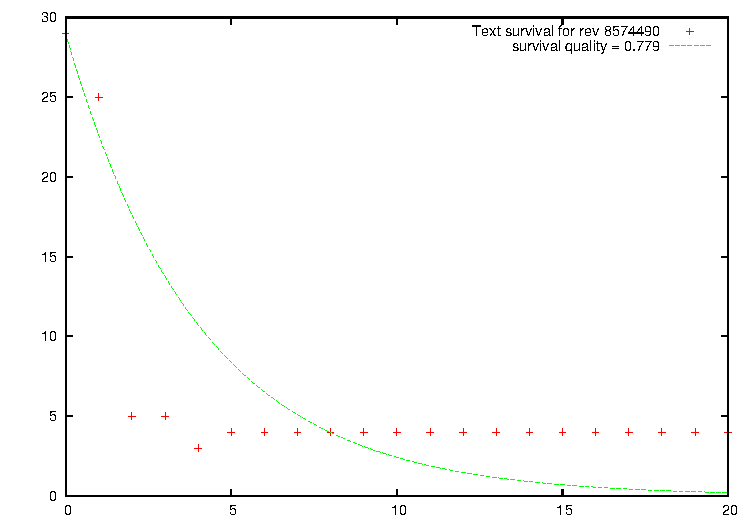
\includegraphics[width=0.45\textwidth]{part-F70-editquality/graph-TS-GeorgeWBush-8574490}}
    \label{fig:ts-GeorgeWBush}
  }
\hspace{1ex}
\subfloat
  [article \underline{Santa Cruz Beach Boardwalk}]
  [The text survival graph for the text initially contributed
	as part of the article \underline{Santa Cruz Beach Boardwalk}.]
  {
    \framebox{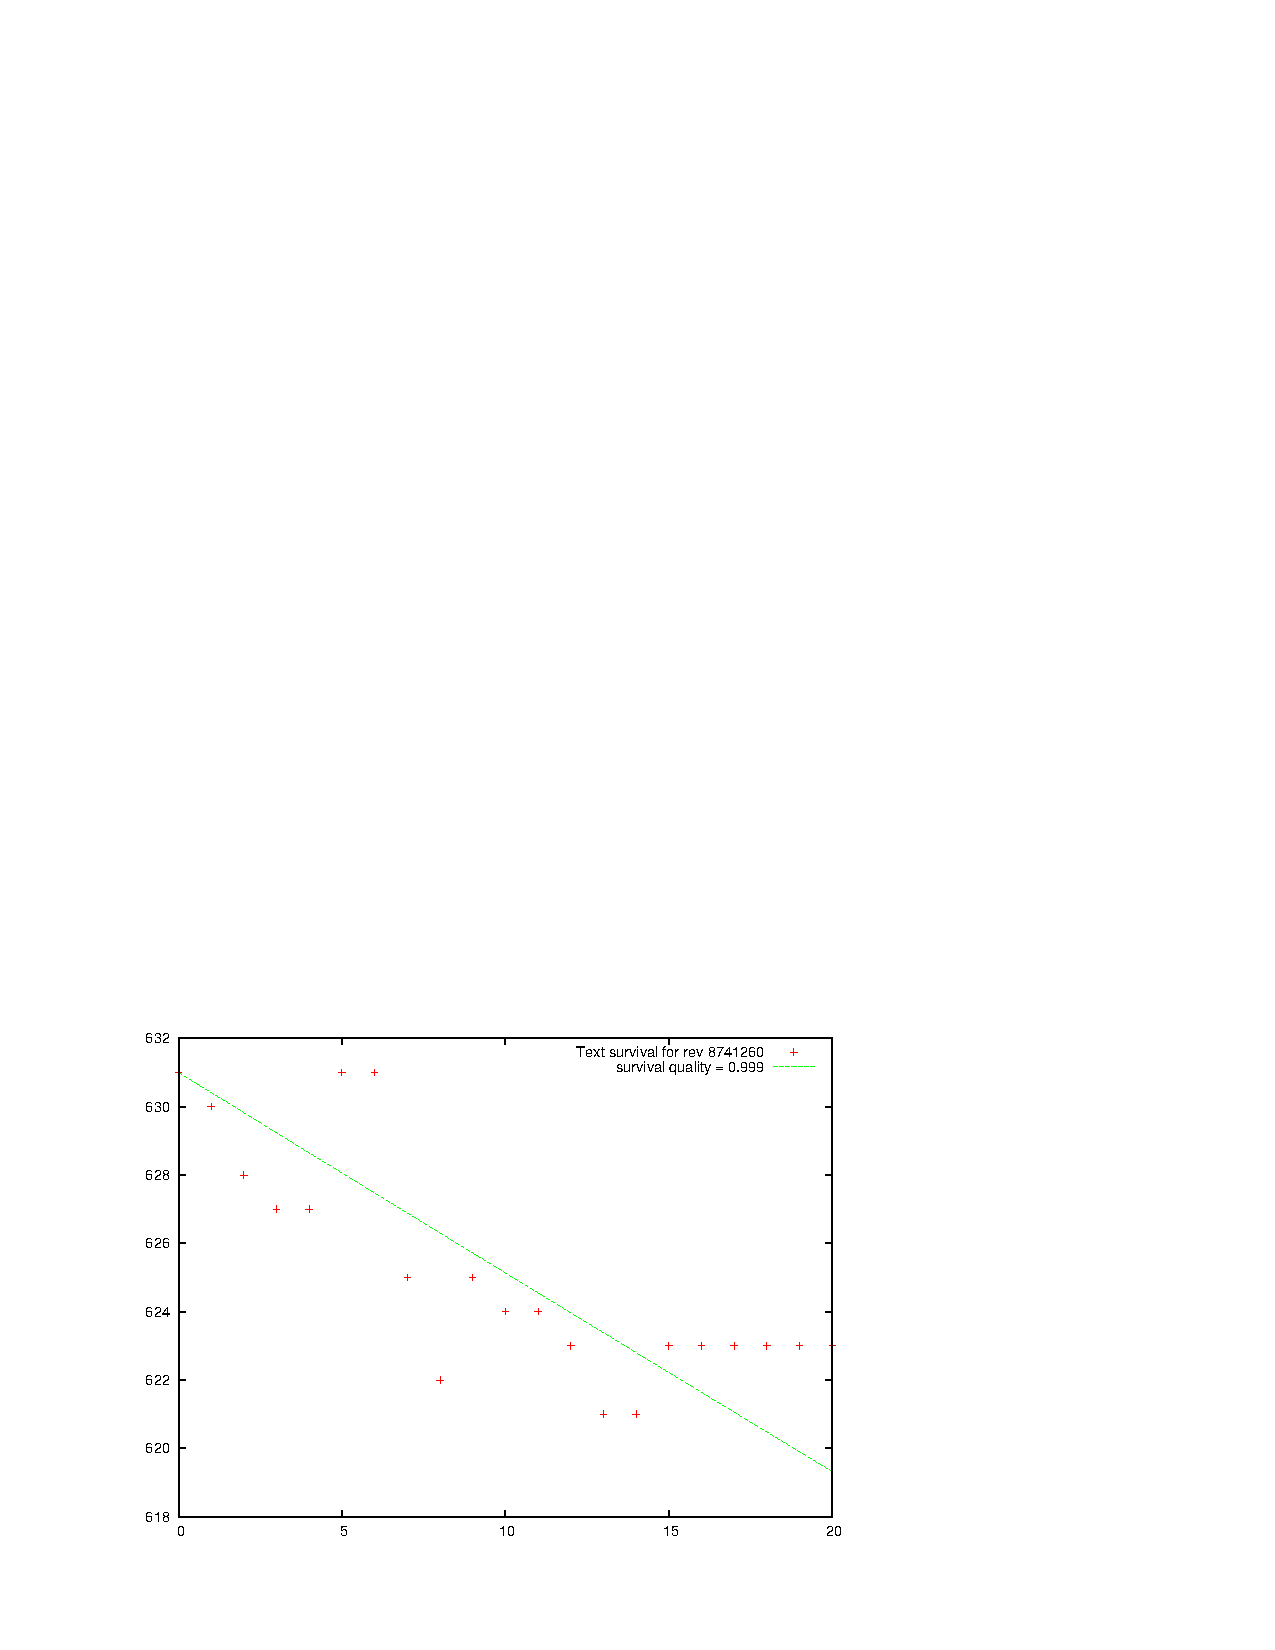
\includegraphics[width=0.45\textwidth]{part-F70-editquality/graph-TS-SantaCruzBeachBoardwalk}}
    \label{fig:ts-SantaCruzBeachBoardwalk}
  }
\caption[The text survival quality graphs for two articles]{
  The text survival quality of two different articles, computed
  based on 20~revisions.
  The majority of the editing happens in the
  revisions immediately after the initial edit, in these two cases.
  \label{fig:ts-GWB-SCBB}
}
\end{figure}

The explanation for this discrepancy turns out to be a flaw in our
thinking about the original model.
While the text survival for contributions does seem to have an
exponential look to it, exponentials do not approach some fixed
non-zero value --- they approach zero.
In order to fit the curve to closely follow the points of text survival,
the last value
(in the case of the data shown in Figure~\ref{fig:ts-GeorgeWBush},
the amount of text that survives after the $20^{th}$ revision)
should be taken as the ``zero reference point'' which is subtracted
from all the values.
Applying our exponential curve fitting technique to these new values
will give a much better approximation to the data.
The problem with this better fit is that it changes the meaning of
a score of zero; instead of meaning that the text was immediately deleted,
a score of zero would mean that the text immediately reached its
final survival level.
In other words, we would be measuring how quickly the text stabilizes,
rather than how much agreement there was that the text belonged in
the article.


\subsection{The Triangle Inequality}
\label{sec:triangle-inequality}

The intuition behind our formulation of edit longevity relies on
the metaphor analogizing the \intro{distance} between two revisions
with the \intro{work} or \intro{effort} that an author puts
into making the edit from one revision to the other;
in particular, it is the triangle inequality (one of the
metric properties of distance) that allows us to say that we
can compute how much effort was \textit{useful} in bringing
the article closer to how it appears in a future revision.

We have explored the use of several different definitions of
the \intro{edit distance} to represent this effort, but
noted that the triangle inequality did not completely hold;
see~\cite{Sankoff1999} for a summary of known conditions under which
the triangle inequality holds for
\intro{listing}, \intro{alignment}, or \intro{trace} distances.

\begin{figure}[htbp]
\centering
  \subfloat[
    listing distance][
    Listing distance is computed by finding the shortest edit script.
    ]{
    \framebox{
      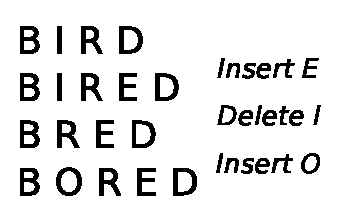
\includegraphics[width=0.4\textwidth]{part-F70-editquality/fig-DiffListing}
    }
  }
  \hspace{2ex}
  \subfloat[
    trace distance
    ][
    Simple trace distance is computed by establishing a correspondence
    between the source and target strings, such that trace lines
    do not cross.
    ]{
    \framebox{
      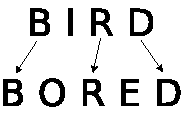
\includegraphics[width=0.4\textwidth]{part-F70-editquality/fig-DiffTrace}
    }
  }
  \\
  \subfloat[
    alignment distance
    ][
    Alignment distance is computed by finding an alignment which
    results in the minimum number of insertions and deletions.
    ]{
    \framebox{
      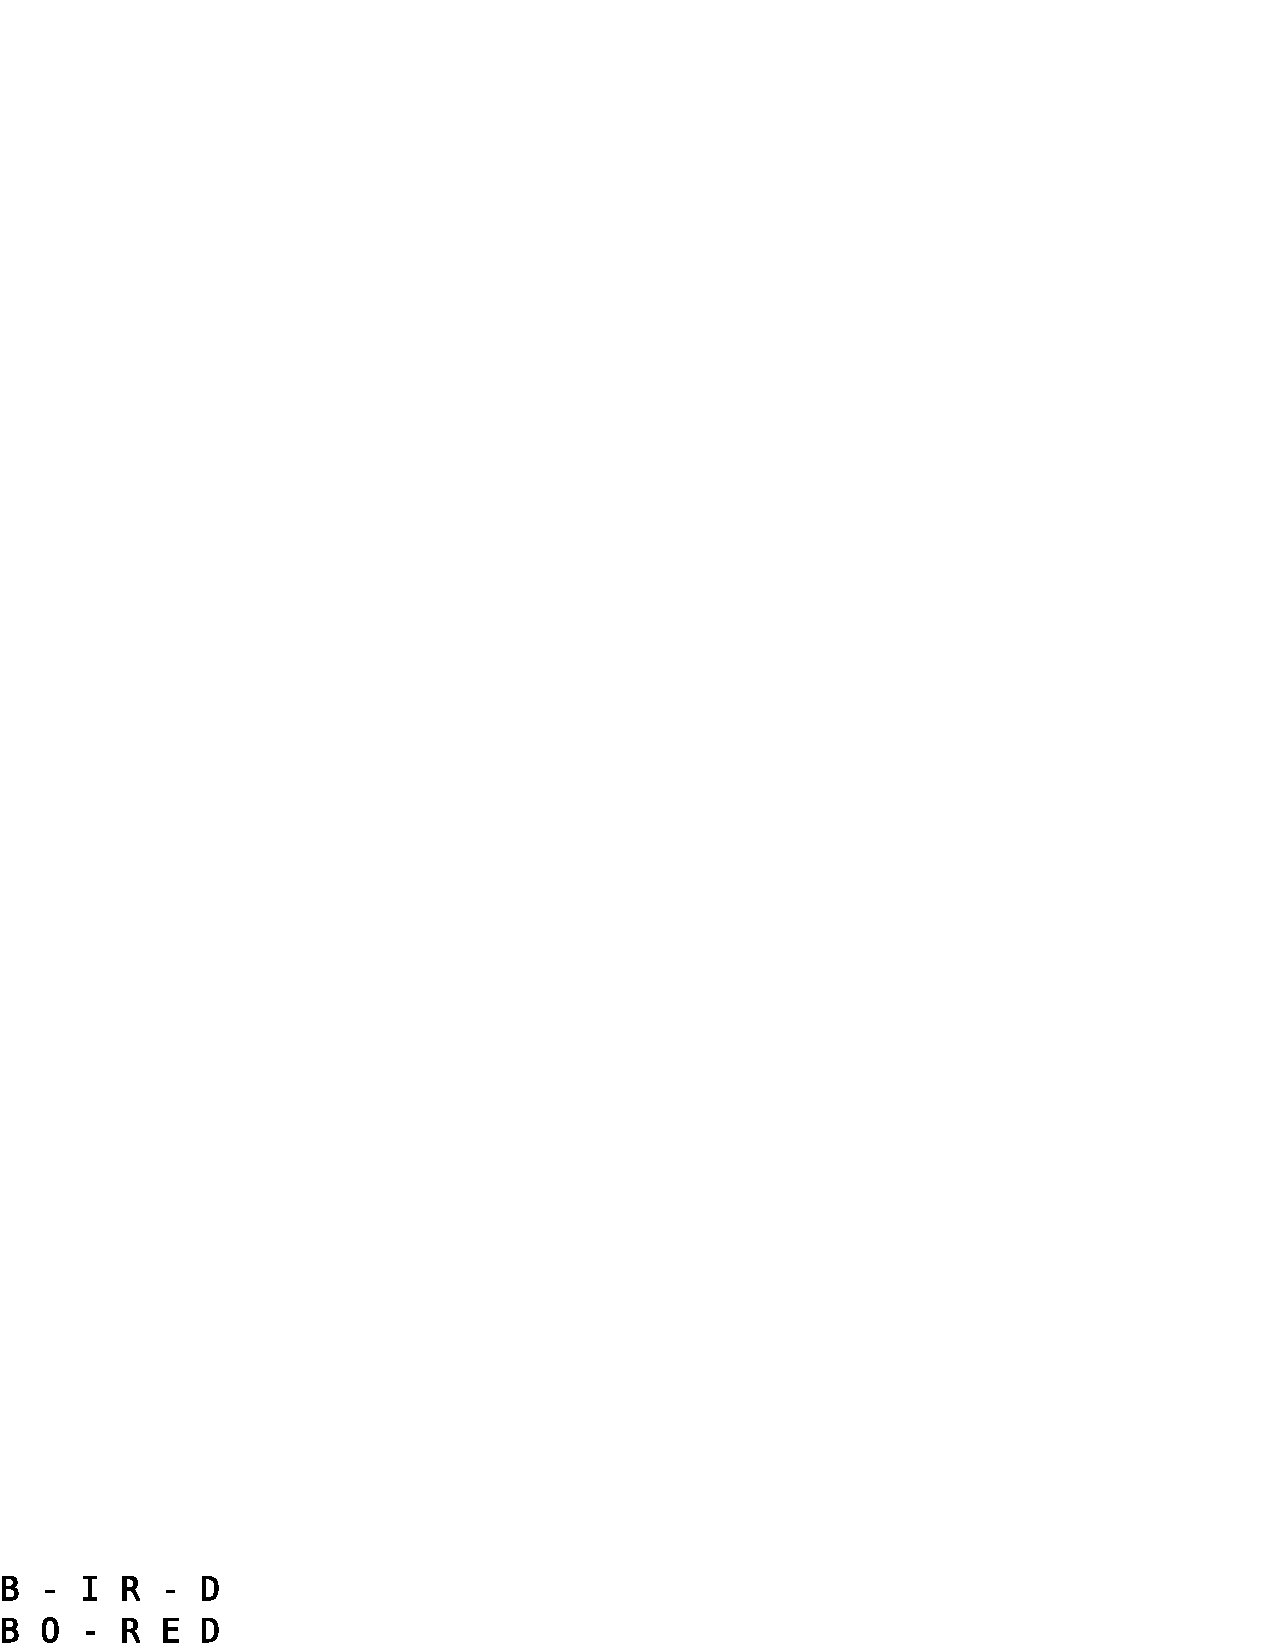
\includegraphics[width=0.4\textwidth]{part-F70-editquality/fig-DiffAlignment}
    }
  }
\caption[Examples of three different styles for computing edit distance]{
  Examples of the three different methods typically used to compute
  edit distance.  See~\cite{Sankoff1999} for an in-depth discussion
  on the distinctions between these methods.
  \label{fig:trace-alignment-listing}
}
\end{figure}

Our particular difference algorithm makes use of
Tichy's block moves~\cite{Tichy1984}, which amounts to computing
the trace that matches the source string to the target string.
That matches are allowed between any parts of the two strings
is equivalent to allowing transpositions as well as the usual
insert and delete operations; the difference we compute does not support
substitutions of one word with another.
There is previous research on allowing
transpositions~\cite{Lowrance1975,Wagner1975,Sankoff1999} in
computing edit distance; our work primarily differs from this
earlier work in that we prefer to select longest matches rather
than minimizing the total edit distance computed.

The various proposals for edit distance that we investigated are
computations derived from the edit script we compute.
Tichy's original counter-example shows that globally greedy algorithms
such as ours do not compute the minimum edit script
(see Figure~\ref{fig:match-comparison}), making it unlikely that
proposed edit distance formulas guarantee the triangle inequality.

\begin{figure}[htbp]
\centering
  \subfloat[
    WikiTrust uses the globally longest match][
    The matching obtained using the WikiTrust method of
      determining all matches and selecting the longest matches first.
    ]{
    \framebox{
      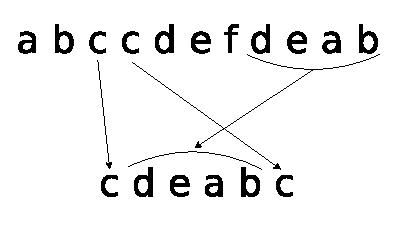
\includegraphics[width=0.4\textwidth]{part-F70-editquality/fig-MatchingGlobal}
    }
  }
  \hspace{2ex}
  \subfloat[
    Tichy uses best match from left-to-right
    ][
    The matching obtained using the Tichy method of scanning
      the target string from left-to-right and selecting
      the longest match found in the source string.
    ]{
    \framebox{
      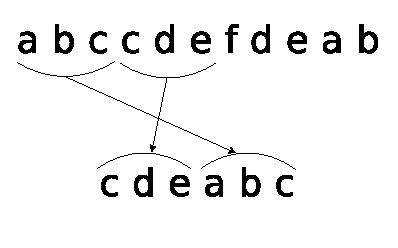
\includegraphics[width=0.4\textwidth]{part-F70-editquality/fig-MatchingLocal}
    }
  }
\caption[An example of when WikiTrust and Tichy differ in matching.]{
  An example of how the matching between a source string and target string
  can differ between WikiTrust's greedy preference for the longest match
  anywhere between the two strings, and Tichy's processing of the
  target string from left-to-right and selecting the longest match
  for the given starting position in the target string.
  This example is based on Tichy's original example demonstrating that
  a globally greedy algorithm does not result in the minimum number of
  operations~\cite{Tichy1984}.
}
\label{fig:match-comparison}
\end{figure}

We present in Appendix~\ref{app:editlong-data} data on the frequency
with which the triangle inequality holds for the various combinations
of difference algorithms and edit distance formulae; only formula~\textbf{ed2}
never violates the triangle inequality.
This is relatively easy to see by an enumeration of the cases, but it
is instructive to examine~\textbf{ed1} first.

To show that~\textbf{ed1} does not satisfy the triangle inequality, we
note that the definition
    \begin{equation*}
    I_{tot} + D_{tot}
    \end{equation*}
is amenable to the \intro{weighted operation} notation used
throughout~\cite{Sankoff1999}.
In this notation, an insertion of word $x$ is said to
contribute weight $w(\phi, x)$ to the final edit distance, and
deletion of word $x$ contributes weight $w(x, \phi)$.
We extend the notation to represent the contribution of a
Move operation on $x$ as $w(x, x)$.
Edit distance~\textbf{ed1} can then be described as the following
assignment of weights:
\begin{align*}
  w(\phi, x) &= 1 \\
  w(x, \phi) &= 1 \\
  w(x, x) &= 0
\end{align*}
For convenience, we represent the situation where a word is in
neither the source nor target revision as $w(\phi, \phi)$ and
assign it a weight of zero.
Note that~\textbf{ed1} assigns a weight of zero to Move operations,
so we do not need to concern ourselves with the location of word~$x$
in the source and target strings.

We consider three revisions, just as we did in analyzing
edit longevity in Figure~\ref{fig-editcontr}: \version{k-1},
\version{k}, and \version{j}.
To verify the triangle inequality,
\begin{equation*}
  \dist{}{k-1,k} + \dist{}{k,j} \ge \dist{}{k-1,j},
\end{equation*}
we enumerate the possible cases of word $x$ existing in each
revision:
\begin{enumerate}
\item word $x$ exists in revision \version{k-1}, but not in
  \version{k} nor \version{j}.
  This translates into deletion operations for \dist{}{k-1,k}
  and \dist{}{k-1,j}, so that we have
  \begin{align*}
    w(x, \phi) + w(\phi, \phi) \ge w(x, \phi),
  \end{align*}
  which is true.
\item word $x$ exists in revision \version{k}, but not in
  \version{k-1} nor \version{j}.
  \begin{align*}
    w(\phi, x) + w(x, \phi) & \ge w(\phi, \phi).
  \end{align*}
\item word $x$ exists in revision \version{j}, but not in
  \version{k-1} nor \version{k}.
  \begin{align*}
    w(\phi, \phi) + w(\phi, x) & \ge w(\phi, x).
  \end{align*}
\item word $x$ exists in revision \version{k-1} and \version{k}, but not in
  \version{j}.
  \begin{align*}
    w(x, x) + w(x, \phi) & \ge w(x, \phi).
  \end{align*}
\item word $x$ exists in revision \version{k-1} and \version{j}, but not in
  \version{k}.
  \begin{align*}
    w(x, \phi) + w(\phi, x) & \ge w(x, x).
  \end{align*}
\item word $x$ exists in revision \version{k} and \version{j}, but not in
  \version{k-1}.
  \begin{align*}
    w(\phi, x) + w(x, x) & \ge w(\phi, x).
  \end{align*}
\item word $x$ exists in all of revisions \version{k-1}, \version{k},
  and \version{j}.
  \begin{align*}
    w(x, x) + w(x, x) & \ge w(x, x).
  \end{align*}
\end{enumerate}

All of these statements are true, so it would seem that
edit distance~\textbf{ed1} satisfy the triangle inequality.
The complication arises in the requirement
that there be a minimum number of words to be considered a
Move operation.
This restriction means that it is possible for a word to exist
in both revisions, but be considered a Deletion and Insertion.
For example, if word $x$ exists in all three revisions, a different
possible analysis is:
  \begin{align*}
    w(x, x) + w(x, x) & \ge w(x, \phi) + w(\phi, x),
  \end{align*}
which does not hold true, and thus the triangle inequality sometimes
will break down.

\bigskip

The proof that edit distance~\textbf{ed2} always satisfies the
triangle inequality follows a similar analysis, but using different
weights:
\begin{align*}
  w(\phi, \phi) &= 0 \\
  w(\phi, x) &= 1 \\
  w(x, \phi) &= 1 \\
  w(x, x) &= 1
\end{align*}
These weights result in every statement holding true, even the
alternative analysis, so that the
full triangle inequality also holds true.

Examining the performance of \textbf{ed2} in
Appendix~\ref{app:editlong-data}, we note that it was far from the best
performing definition of edit distance in terms of predicting vandalism
in the PAN-WVC-10 dataset.
Although using an edit distance formulation that satisfies the triangle
inequality is desirable, it is not sufficient to achieve good
performance.
The goal of an edit distance function in our context is to estimate
the amount of \intro{effort} that an author expends in creating an
edit from one revision to another.
We chose to follow a model which prefers the longest possible match
between source and target revisions, but another viable route is to
minimize the amount of text which is rearranged (\ie minimize the
number of transpositions)~\cite{Wagner1975}.
We leave as an open question how to best characterize the work
that an author does.


\section{Conclusions}

We propose two measures of revision quality computed
from Wikipedia's revision history.
The measure \textit{text longevity} is based on an intuitive
model of computing the text added by authors at each revision
and detecting how much of that text remains within the article
in subsequent revisions; to account for the variation in
the amount of preserved text over the subsequent revisions,
we model the change as a geometrically decaying process
and compute the decay rate as a single value to describe
the variation.
The measure \textit{edit longevity} was developed to address
the reality that authors also delete and rearrange text,
and that these are valuable contributions to the Wikipedia.
We use edit distance~\cite{Levenshtein1966} to describe the
amount of \intro{effort} that an author puts into making a
revision to an article; this is the basis for computing
edit longevity, which estimates the amount of effort by an
author that brings the article text closer to some future
version of the article.

We evaluate these two measures using the PAN-WVC-10 dataset, which is
manually annotated to indicate which revisions are vandalism and which
are well-intentioned edits, and treat each as a predictor of vandalism.
We find that edit longevity performs much better than text longevity,
but even text longevity does better than chance at predicting vandalism.
Overall, these results are encouraging for using edit longevity and text
longevity as signals for inferring the community feedback of an author's
edit.  Knowing the quality of edits, we can build an author reputation
system upon these signals; we describe such a system in
Chapter~\ref{ch:reputation}.



